\documentclass[border=20pt]{standalone}

\usepackage{tikz}
\usepackage{ifthen}
\usetikzlibrary{arrows, positioning, calc}
\usetikzlibrary{shapes.multipart} 

\usepackage{incgraph}
\usepackage{standalone}
\begin{document}
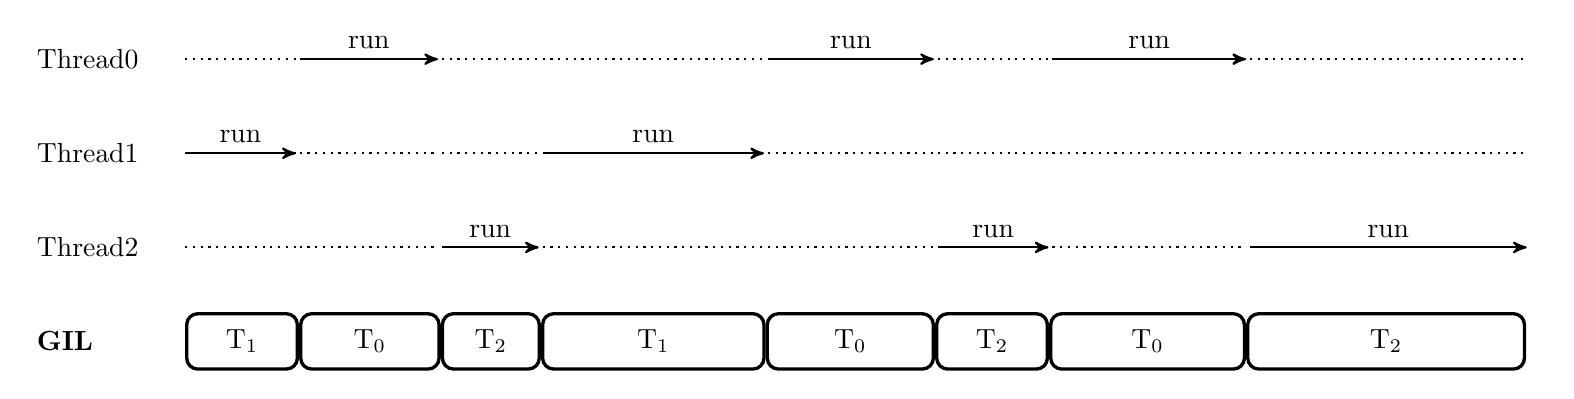
\begin{tikzpicture}

\def\iotext{numpy}

\tikzset{
    %Define standard arrow tip
    >=stealth',
    %Define style for boxes
    rbox/.style={
           rectangle,
           fill=white,
           rounded corners,
           draw=black, very thick,
           text width=2em,
           minimum height=2em,
           text centered},
    run/.style={
           ->,
           thick
    },
    wait/.style={
           dotted,
           thick
    },
};

%nodes

\node[text width=5em] (thread0) {Thread0};
\node[below=2em of thread0, text width=5em] (thread1) {Thread1};
\node[below=2em of thread1, text width=5em] (thread2) {Thread2};
\node[below=2em of thread2, text width=5em] (gil) {\bf GIL};

\pgfmathsetseed{42}

\edef\i{0}
\pgfmathparse{random(0, 2)}
\edef\i{\pgfmathresult}

\foreach \x in {4em, 5em, 3.5em, 8em,  6em, 4em,  7em, 10em}{

\pgfmathparse{int(mod(\i+random(1, 2), 3))};
\xdef\i{\pgfmathresult}

\node[right=\x of thread0] (t0) {};
\node[right=\x of thread1] (t1) {};
\node[right=\x of thread2] (t2) {};
\node[right=\x of gil] (gil1) {};

\draw[wait] (thread0) -- (t0);
\draw[wait] (thread1) -- (t1);
\draw[wait] (thread2) -- (t2);
\draw[run] (thread\i) -- (t\i) node[midway, above] {run};


\node[right=\x of thread0, inner sep=0em] (thread0) {};
\node[right=\x of thread1, inner sep=0em] (thread1) {};
\node[right=\x of thread2, inner sep=0em] (thread2) {};
\node[right=0em of gil, rbox, text width=\x, inner sep=0em] (gil) {T$_\i$};

}





% Draw a centered plus sign

\end{tikzpicture}
\end{document}